\documentclass[12pt]{beamer}
%\usetheme{CambridgeUS} 
\usetheme{Madrid} 
%\usetheme{Berkeley}
\usepackage{graphicx}
\usepackage{multirow}
\usepackage{multicol}
\usepackage{booktabs}
\usepackage{tabularx}
\usepackage[utf8x]{inputenc}
\usepackage[alf]{abntex2cite}	% Citações padrão ABNT
\usepackage[brazilian,hyperpageref]{backref}	 % Paginas com as citações na bibl
\usepackage{tcolorbox}

\setbeamertemplate{caption}[numbered]


% nova lista de itens
\newenvironment{itens}{\itemize\addtolength{\itemsep}{0.55em}\vspace{0.3em}}{\enditemize}
\newcommand{\incr}[2]{#1 += #2}
\newcommand{\decr}[2]{#1 -= #2}

\newcommand\SourcePadrao{José Eleandro Custódio, 2018}
\newcommand{\selectFont}{\fontsize{2.7mm}{4.0mm}\selectfont}


\title{Atribuição autoral de textos digitais}
\author
	[J.~E.~Custódio]
	{José Eleandro Custódio}
\institute
	[\hypersetup{urlcolor=jdwhite}
	%\href{http://www.ppgsi.each.usp.br/}{PPgSI} %
	\href{http://www.usp.br/}{USP}]
	%{Orientador: Prof. Dr. Ivandré Paraboni \\ ~ \\
	{Programa de Mestrado em Sistemas de Informação - PPgSI\\%
		Universidade de São Paulo - USP}
\date
	[11/2018]
	{Novembro de 2018}

\begin{document}

\maketitle


% \section{Conteúdo}
% \frame{\tableofcontents}
% \section{Oba}
\fontsize{3mm}{4mm}\selectfont
\setbeamerfont{block title}{size=\scriptsize}


%*********
\begin{frame}{Informações gerais}
\fontsize{3.0mm}{4.0mm}\selectfont

\begin{itemize}
	\item {\bf Orientador:} Prof. Dr. Ivandré Paraboni
	\item {\bf Semestre no curso:} 4o.
	\item {\bf Qualificação:}  29/10/2018
	\item {\bf Defesa:} realização planejada para 30/06/2019
	\item {\bf Linha de pesquisa:} Inteligência de sistemas
	\item {\bf Área de pesquisa:} Inteligência artificial
	\item {\bf Área de aplicação:} Linguística computacional / Língua natural
\end{itemize}

\end{frame}
%*********


\begin{frame}{Agenda}
	\tableofcontents
\end{frame}

\section{Introdução}

\begin{frame}{Introdução}
	\begin{alertblock}{Contexto}
		\begin{itemize}\itemsep9pt
		\item A atribuição autoral de textos digitais (AA) (do inglês, {\it Authorship Attribution})  visa identificar quem é o autor de um determinado texto a partir de um conjunto de autores possíveis \cite{Potthast2017}.
		
		\item A premissa principal da AA é que o autor deixa rastros de seu estilo, sendo que esses rastos podem ser a preferência por certas palavras, o tamanho do vocabulário, a utilização de pontuação e a repetição de certos elementos gramaticais.
		
		\item Quantificar essas informações é uma tarefa conhecida por estilometria \cite{Stamatatos2009}.
		
		\end{itemize}
	
		
	\end{alertblock}

\end{frame}

\begin{frame}{Aplicações da Atribuição Autoral}

\begin{columns}
	\begin{column}{0.65\textwidth}
		\begin{alertblock}{Aplicações da AA}
			Sua aplicação pode ajudar: 
			\begin{itemize}\itemsep9pt
				\item  em casos de escândalos de corrupção, como no caso Enron
				 \cite{corpusEnron,Chen2011}.
				\item na identificação de abusos na utilização da internet \cite{Gillam2012quite}.
				\item na detecção de notícias falsas \cite{Peng2016}.
				\item na detecção de casos onde uma pessoa tenta se passar por outra \cite{Koppel2018_pseud}.
				\item na atribuição autoral de código-fonte \cite{Alsulami2017}
				\item na detecção de pseudônimos \cite{Juola15}
				
			\end{itemize}
		\end{alertblock}
	\end{column}
	\begin{column}{0.3\textwidth}  %%<--- here
		\begin{alertblock}{Área de interesse}
			\begin{itemize}
				\item Humanidades Digitais
				\item Análise Forense
				\item Linguística computacional
			\end{itemize}
		\end{alertblock}
	\end{column}
\end{columns}

\end{frame}


\begin{frame}{Métodos para atribuição autoral}

Os métodos computacionais para atribuição autoral utilizam: 
\begin{itemize}
  \item Análise estatística multivariada \cite{Savoy2016,AA_delta2017}.
  \item Métodos baseados em vizinho mais próximo \cite{Kocher2017Verificacao,Koppel2018_pseud,Varela2016}.
  \item Aprendizado de máquina com SVM \cite{Schwartz2013,aa-distortion}.
  \item Redes neurais recorrentes \cite{Bagnall2016}.
  \item Redes neurais de convolução \cite{Shrestha2017,Sari2016}.
  modelos de compressão \cite{Halvani2018}
\end{itemize}

\end{frame}

\section{Conceitos}

\begin{frame}{Definições}
\begin{block}{Definições}
	\begin{itemize}\itemsep9pt
		\item A atribuição autoral (AA) é uma técnica computacional que visa identificar o autor de um texto a partir de um conjunto de autores possíveis, baseando-se em padrões de estilo deixados pelos autores \cite{Potthast2017}.
		
		\item Do ponto de vista de aprendizado de máquina, a AA pode ser vista como um problema de classificação multi-classes \cite{Stamatatos2009}.
		
		\item A quantificação do estilo de escrita, ou estilometria, compreende um vasto conjunto de medidas e técnicas que buscam extrair uma ``biometria'' textual \cite{Neal2017}.
	\end{itemize}
\end{block}

\begin{block}{}
	Apesar da similaridade com a tradicional tarefa de classificação de documentos, a AA busca elementos inconscientes da escrita que sejam independentes do conteúdo semântico do texto \cite{Keselj2003}.
\end{block}

\end{frame}


\begin{frame}{Conceitos - Fatores que influenciam a AA}

\begin{columns}
	\begin{column}{0.48\textwidth}
		\begin{tcolorbox}[title=Canal,height=2.4cm,valign=center]\selectFont
			$\bullet$ E-mail, jornais, livros, SMS
			
			$\bullet$ Textos mais ou menos formais.                    
		\end{tcolorbox}
	\end{column}
	\begin{column}{0.48\textwidth}
		\begin{tcolorbox}[title=Idioma,height=2.4cm,valign=center]\selectFont
			$\bullet$ Complexidade morfológica e lexical diferentes.
		\end{tcolorbox}
	\end{column}
\end{columns}
\begin{columns}
	\begin{column}{0.48\textwidth}
		\begin{tcolorbox}[title=Tópico,height=2.4cm,valign=center]\selectFont
			$\bullet$ Economia, celebridades, dia-a-dia
			
			$\bullet$ Influencia o vocabulário.                    
		\end{tcolorbox}
	\end{column}
	\begin{column}{0.48\textwidth}
		\begin{tcolorbox}[title=Domínio ou Gênero do texto,height=2.4cm,valign=center]\selectFont
			$\bullet$ Contos, artigos, avaliações de produtos
			
			$\bullet$ Influencia no rigor formal e no vocabulário.
		\end{tcolorbox}
	\end{column}
\end{columns}

\begin{columns}
	\begin{column}{0.48\textwidth}
	\begin{tcolorbox}[title=Tamanho do texto,height=2.4cm,valign=center]
		$\bullet$ Métodos probabilísticos são afetados pelo número de observações.                  
	\end{tcolorbox}
	\end{column}
	\begin{column}{0.48\textwidth}
	\begin{tcolorbox}[title=Número de autores,height=2.4cm,valign=center]
		$\bullet$ O aumento do número de classes requer o aumento do número de classes.                    
	\end{tcolorbox}
	\end{column}
\end{columns}

\end{frame}






%%%%%%%%%%%%%%%%%%%%%%%%%%%%%%%%%%%%%%%%%%%%%%%%%%%%%%%
\begin{frame}{Conceitos - Subtarefas da análise autoral}
	\begin{columns}
		\begin{column}{0.48\textwidth}
			\begin{tcolorbox}[colback=red!5!white,colframe=red!75!black,title=AA de conjunto fechado,height=2.4cm,valign=center]\selectFont
				Os textos do conjunto de teste pertencem a um dos autores candidatos presentes no córpus de treinamento.                    
			\end{tcolorbox}
		\end{column}
		\begin{column}{0.48\textwidth}
			\begin{tcolorbox}[title=AA de conjunto aberto,height=2.4cm,valign=center]\selectFont
				Os textos do conjunto de teste não necessariamente foram escritos por um dos autores do córpus de treinamento                    
			\end{tcolorbox}
		\end{column}
	\end{columns}
	
	\begin{columns}
		\begin{column}{0.48\textwidth}
			\begin{tcolorbox}[title=K-Atribuição ou ordenação ,height=2.4cm,valign=center]\selectFont
				As saídas do classificador são ordenadas pela probabilidade e são retornados os K autores mais prováveis.
			\end{tcolorbox}
		\end{column}
		\begin{column}{0.48\textwidth}
			\begin{tcolorbox}[title=Caracterização,height=2.4cm,valign=center]\selectFont
				São extraídas informações demográficas do autor do texto podem reduzir a lista de candidatos.                    
			\end{tcolorbox}
		\end{column}
	\end{columns}
	
	\begin{columns}
		\begin{column}{0.48\textwidth}
			\begin{tcolorbox}[colback=green!5!white,colframe=green!75!black,title=Verificação,height=2.4cm,valign=center]\selectFont
				Verifica-se se dois documentos foram escritos pelo mesmo autor, não sendo necessário saber quem são os autores.                
			\end{tcolorbox}
		\end{column}
		\begin{column}{0.48\textwidth}
			\begin{tcolorbox}[title=Demais,height=2.4cm,valign=center]\selectFont
				Agrupamento, Ligação e Quebra de estilo.                    
			\end{tcolorbox}
		\end{column}
	\end{columns}

\end{frame}


%%%%%%%%%%%%%%%%%%%%%%%%%%%%%%%%%%%%%%%%%%%%%%%%%%%%%%%
\begin{frame}{Conceitos - Tipos de conhecimentos usados}

A abordagem estilométrica tradicional utiliza as seguintes fontes de conhecimento:

\begin{itemize}
	\item {\bf Categoria lexical:} tamanho médio das palavras, número de letras maiúsculas, quantidade de dígitos, tamanho das sentenças, etc.
	
	\item {\bf Categoria sintática:} frequência da pontuação, palavras de função, frases começando com maiúscula, etc.
	
	\item {\bf Categoria semântica:} contagem das palavras, analisadores semânticos, {\it word embeddings}, etc.
	
	\item {\bf Categoria estrutura:} indentação, tamanho do parágrafo, etc.
	
	\item {\bf Categoria específica de domínio:} palavras-chave, {\it tags} HTML, {\it emoticons}, nomes de produtos.
\end{itemize}
\end{frame}


%%%%%%%%%%%%%%%%%%%%%%%%%%%%%%%%%%%%%%%%%%%%%%%%%%%%%%%
\begin{frame}{Conceitos - Tipos de conhecimentos usados}

Outra classificação possível e simplificada dos conhecimentos utilizados na AA pode ser a utilização das famílias baseadas em palavras e caracteres.


\begin{tcolorbox}[colback=blue!1!white,colframe=blue!35!black,title=Palavras,valign=center]
	\begin{itemize}
		\item As palavras mais frequentes são independentes de domínio e utilizadas de forma inconsciente \cite{Kestemont2014}.
		\item {\bf Palavras de função} (do inglês, {\it function words}) compreende artigos, preposições, locuções adverbiais, e outros.\\
		\item Capturam semântica e elementos de conexão entre sentenças.
		\item Diversas ferramentas são preparadas para usar a unidade {\it palavra}.
	\end{itemize}			
\end{tcolorbox}

\end{frame}

%%%%%%%%%%%%%%%%%%%%%%%%%%%%%%%%%%%%%%%%%%%%%%%%%%%%%%%
\begin{frame}{Conceitos - Tipos de conhecimentos usados}\selectFont

	\begin{tcolorbox}[colback=green!1!white,colframe=green!35!black,title=Caracteres,valign=center]
		\begin{itemize}
			\item As sequências de caracteres são considerados os modelos mais efetivos para AA \cite{KjellWF94,Neal2017}.
			\item Os {\bf caracteres mais frequentes (CNG)} (do inglês, {\it common n-grams}) \cite{Keselj2003,Sapkota2014}.
			\item São independentes de idioma.
			\item Não precisam de {\it stemming} pois lidam bem com idiomas flexionais.
			\item Geram vetores de contagem mais densos que os vetores de palavras.
			\item Os n-gramas de caracteres conseguem capturar pontuação, utilização de espaços, preferências temporais, palavras de função de tamanho curto.
			\item O trabalho em \citeonline{aa-Sapkota2015} mostra que apesar de independente de idioma nem todos os {\it char n-gramas} tem a mesma origem.
		\end{itemize}

	\end{tcolorbox}
\end{frame}

%%%%%%%%%%%%%%%%%%%%%%%%%%%%%%%%%%%%%%%%%%%%%%%%%%%%%%%
\begin{frame}{Conceitos - Modelos computacionais}
\begin{tcolorbox}[title=Modelo tradicional de representação textual - BOW,valign=center]\selectFont
	\begin{itemize}
		\item Hipótese distribucional aplicada a documentos \cite{Turney2010}
		\item Modelo de n-gramas
		\item Conhecimentos: Caracteres, Palavras, POS
		\item TF-IDF
		\item TF-IDF equações alternativas utilizadas nos experimentos:
			\begin{itemize}\selectFont
				\item $ TF_{sublinear} = 1 + \log TF_{t,d}$  $\longrightarrow$ Definição I do SMART. 
				\item $
				IDF_{Suavizado}(t,D) = log\left (
				\frac{D}{DF(t)}
				\right ) + 1
				$
			\end{itemize}
	\end{itemize}	
\end{tcolorbox}
\end{frame}


\begin{frame}{Conceitos - Modelos computacionais}
\selectFont
\begin{columns}
	\begin{column}{0.60\textwidth}
		\begin{tcolorbox}[title=Modelo de representação distribuída,height=7cm,valign=center]\selectFont
			\begin{itemize}
				\item Hipótese distribucional aplicada símbolos
				\item Modelos neurais de língua natural \cite{Bengio2003}
				\item Aprendizado não supervisionado
				\item Transferência de conhecimento
				\item {\it Word embeddings} 
				\begin{itemize}\selectFont
					\item Representa cada palavra, ou símbolo, em k dimensões, sendo k menor que o tamanho do vocabulário.
					\item Word2Vec \cite{Mikolov2013}
					\item Doc2Vec \cite{QuocLe2014}
					\item FastText \cite{bojanowski2017enriching}
				\end{itemize}
			\end{itemize}
		\end{tcolorbox}		
	\end{column}
	\begin{column}{0.40\textwidth}
		\begin{tcolorbox}[title=Modelo Word2Vec,height=7cm,valign=center]\selectFont
			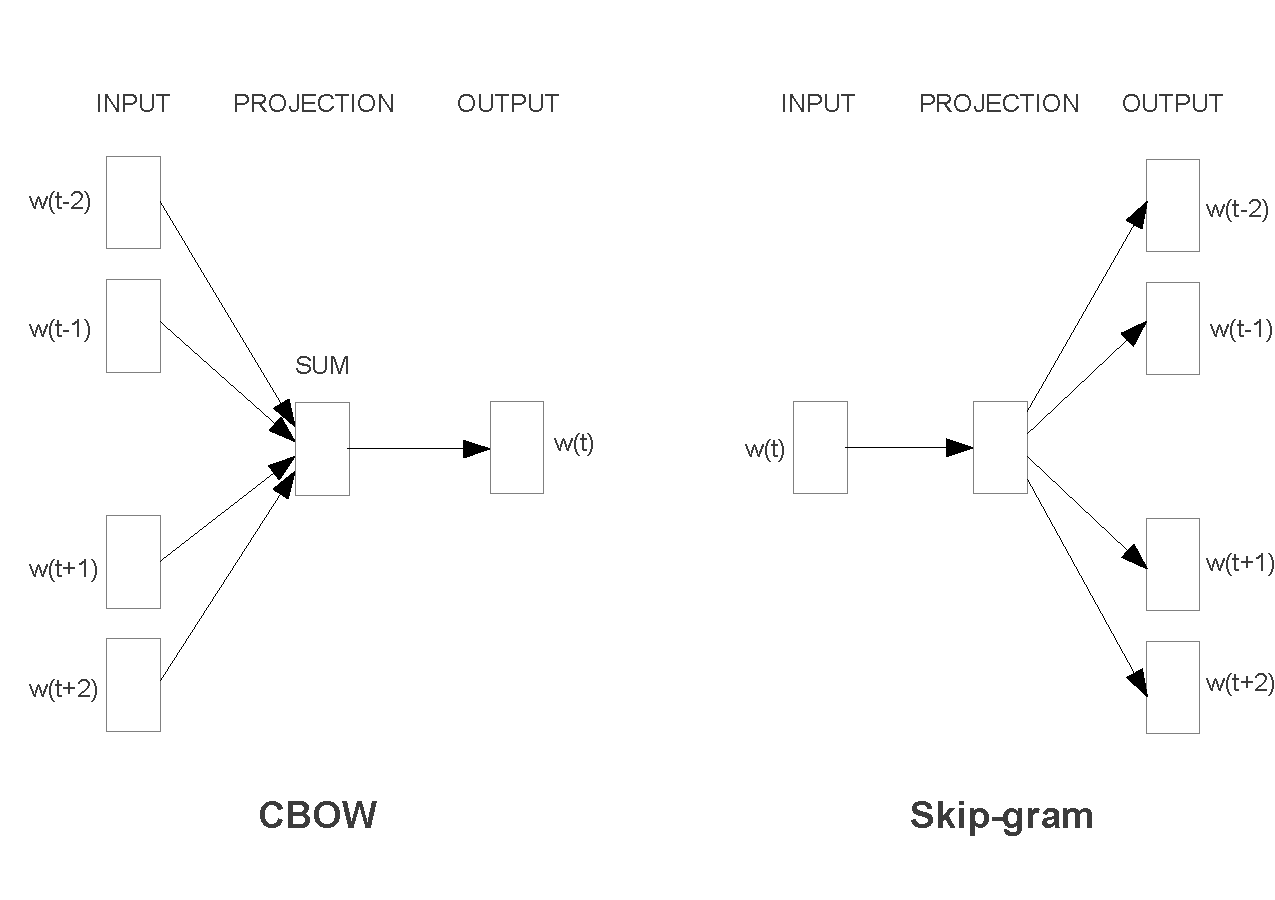
\includegraphics[trim=350 20 0 20,clip,width=.95\textwidth]{images/efficient-models.pdf}
			Fonte: \citeonline{Mikolov2013}
		\end{tcolorbox}		
	\end{column}
\end{columns}
\end{frame}




\begin{frame}{Modelos computacionais baseados em distância}
\selectFont
	As medidas, ou funções, de distância devem obedecer quatro propriedades \cite{deza2009encyclopedia}:
	\begin{enumerate}\selectFont
		\item $D(A,B) >= 0 $ para todo $A$ e $B$, D é positiva.
		\item $D(A,B) = 0 $ se e, somente se, $A = B$.
		\item $D(A,B) = D(B,A) $, $D$ é uma função simétrica.
		\item $D(A, C) <= D(A, B) + D(B, C)$, a desigualdade triangular.
	\end{enumerate}


	\begin{columns}
	\begin{column}{0.48\textwidth}
		\begin{tcolorbox}[colback=red!5!white,colframe=red!75!black,title=Distância de cosseno,height=2cm,valign=center]\selectFont
			$
			Cossenos \left ( A,B \right ) = 1 -\frac{A\cdot B}{\left \| A \right \| \left \| B \right \|}
			$            
		\end{tcolorbox}
	\end{column}
	\begin{column}{0.48\textwidth}\selectFont
		\begin{tcolorbox}[title=Manhattan,height=2cm,valign=center]\selectFont
			$
			Manhattan \left ( A,B \right )= \sum_i {\left| A_i - B_i \right|}
			 $     
	\end{tcolorbox}
	\end{column}
	\end{columns}


	\begin{columns}
		\begin{column}{0.48\textwidth}
			\begin{tcolorbox}[colback=blue!5!white,colframe=blue!75!black,title=Jaccard,height=2cm,valign=center]\selectFont
			$
			Jaccard(A,B) = \frac{\left | A \cap B \right |}{\left | A \cup B \right |}
			$
			
			Interseção binária
			\end{tcolorbox}
		\end{column}
		\begin{column}{0.48\textwidth}\selectFont
			\begin{tcolorbox}[title={MinMax, ou Jaccard generalizado},height=2cm,valign=center]\selectFont
				$
				MinMax (A,B) = \frac{ \sum_{i}^{n}{ min(A_i,B_i|}}{\sum_{i}^{n}{max(A_i,B_i)}}
				$      
			\end{tcolorbox}
		\end{column}
	\end{columns}

\end{frame}


\begin{frame}{Modelos computacionais baseados em distância}
\selectFont
\begin{tcolorbox}[colback=blue!5!white,colframe=blue!75!black,valign=center,title=Regra $\Delta$ de Burrows ]\selectFont
	\begin{equation}
	\begin{aligned}
	\Delta Burrow \left ( A, B \right) = \frac{1}{N}\sum_{i=1}^{N}\left | Zscore(A_i,C_i) - Zscore(B_i,C_i) \right |
	\\
	Zscore(X_i,C_i)= \frac{X_i - \mu (C_i) }{\sigma(C_i)}
	\end{aligned}
	\label{eq:deltaBorrow}
	\end{equation}
		
	Distância de Manhattan dos Z-score das frequências         
\end{tcolorbox}


	\begin{columns}
	\begin{column}{0.48\textwidth}
		\begin{tcolorbox}[title=Keselj,height=2cm,valign=center]\selectFont
			$
			Keselj (A,B) = \sum_i^n \left ( \frac{ 2*\left(A_i-B_i \right ) }{A_i+B_i}\right )^{2}
			$
		\end{tcolorbox}
	\end{column}
	\begin{column}{0.48\textwidth}\selectFont
		\begin{tcolorbox}[title=Stamatatos,height=2cm,valign=center]\selectFont
			$
Stamatatos (A,B, C) = \sum_i^n \left ( \frac{ 2*\left(A_i-B_i \right ) }{A_i+B_i}\right )^{2} * \left ( \frac{ 2*\left(A_i-C_i \right ) }{A_i+C_i}\right )^{2}
			$      
		\end{tcolorbox}
	\end{column}
\end{columns}

Onde A e B são vetores de frequências documentos que se desejam comparar e C é o vetor de frequência do córpus.

\end{frame}


\begin{frame}{Modelos computacionais baseados em distância}
	\begin{tcolorbox}[colback=blue!5!white,colframe=blue!75!black,title=Distância Komogorov-Smirnov,height=5cm,valign=center]\selectFont
		\selectFont
		\begin{center}
			\begin{figure}[]
				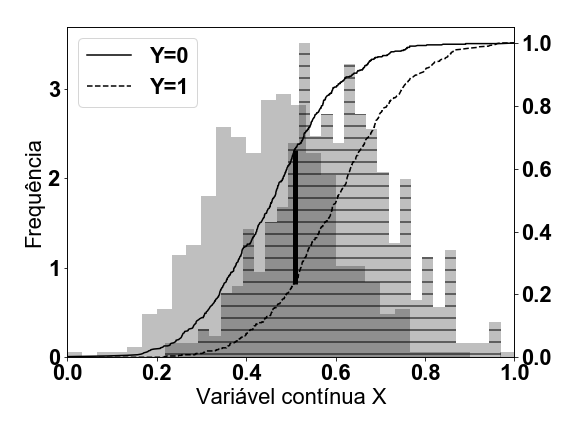
\includegraphics[scale=0.20]{images/KS_teorico.png}
				\label{fig:ksTeorico}
			\end{figure}
			Fonte: \SourcePadrao
		\end{center}
	\end{tcolorbox}


	\begin{tcolorbox}[colback=blue!5!white,colframe=blue!75!black,title=Definição e propriedades,valign=center]\selectFont
	\begin{itemize}
		\item $KS(X,Y) = \operatorname*{arg\_max}_x abs(CDF(x | y=0)- CDF(x | y=1))$
		\item Distância entre as curvas de probabilidades acumuladas.
		\item Mede se a variável binária representa distribuições diferentes.
	\end{itemize}
	\end{tcolorbox}
\end{frame}


\begin{frame}{Modelos de aprendizado de máquina (AM)}

\begin{columns}
	\begin{column}{0.55\textwidth}
		\begin{tcolorbox}[colback=blue!5!white,colframe=blue!75!black,valign=center,title=Regressão logística softmax]\selectFont
			\centering
			\begin{equation} 
			\begin{matrix}
			f_1(X) - \ln Z  & = \ln P(Y=1|X) \\
			\cdots & \cdots \\
			f_c(X) - \ln Z & = \ln P(Y=c|X) \\
			\end{matrix}
			\label{eq:logisticaArray}
			\end{equation}
			
			$\Downarrow$
			
			\begin{equation}
			P(Y=c|X) =softmax(X,c) = \frac{e^{f_c(X)}}{\sum_{k=1}^{K} e^{f_k(X)}}
			\label{eq:softmax}
			\end{equation}
		\end{tcolorbox}
	\end{column}
	\begin{column}{0.45\textwidth}
		\begin{tcolorbox}[colback=blue!5!white,colframe=blue!75!black,valign=center,title=Propriedades]\selectFont
			$\bullet$ Não assume a independência das variáveis.
			
			$\bullet$ Possui saída probabilística.
			
			$\bullet$ As probabilidades reflem o balanceamento das classes.
			
			$\bullet$ Possui saída contínua.
			
			$\bullet$ É um classificador linear.
			
			$\bullet$ É usado em aprendizado profundo.
		\end{tcolorbox}
	\end{column}
\end{columns}

\end{frame}
\section{Trabalhos relacionados}

\begin{frame}{Trabalhos selecionados}
\setlength{\tabcolsep}{5pt}\selectFont
\begin{table}[]
	\caption{Trabalhos selecionados}
	\begin{tabular}{lllll}
		\toprule
		{ Estudo}                   & {  Idioma}     & { Tarefa} & {  Conhecimento}      & {  Método}           \\ \toprule
		\citeonline{aa-Sapkota2015} & EN             & A         & {\it C}               & SVM                  \\ \hline
		\citeonline{aa-distortion}  & EN             & A,V       & {\it C, W}            & SVM                  \\ \midrule
		\citeonline{Schwartz2013}   & EN             & A         & {\it C, W}            & SVM                  \\ \hline
		\citeonline{aa-rocha-2017}  & EN             & A,V       & {\it C, W, P}         & {\it SVM}, RF e SCAP \\ \midrule
		\citeonline{AA_delta2017}   & EN             & C         & {\it W}               & Clusterização        \\ \hline
		\citeonline{Varela2016}     & PT-BR          & A,V       & {\it P}               & SVM                  \\ \hline
		\citeonline{posadas2017}    & EN             & A         & D2V de {\it W}        & Softmax e SVM        \\ \hline
		\citeonline{RhodesCS224D}   & EN             & A         & W2V                   & CNN-Softmax          \\ \hline
		\citeonline{Shrestha2017}   & EN             & A         & {\it C One-hot}       & Softmax              \\ \hline
		\citeonline{Bagnall2016}    & PAN2015 & C         & {\it C One-hot}       & RNN-Softmax          \\ \bottomrule
	\end{tabular}
	\label{tab:revisao_sumarizacao_geral}
	\SourcePadrao
\end{table}
\end{frame}
\section{Experimentos}

\begin{frame}{Experimentos}
\begin{alertblock}{Experimentos}
\end{alertblock}
\end{frame}

%*******************************************************************
\begin{frame}{Experimento 1: Verificação autoral}
\fontsize{3.0mm}{4.0mm}\selectfont
\begin{block}{Publicação 1}
	CUSTÓDIO, J. E.; PARABONI, I. Similaridade de Textos aplicada à Verificação Autoral.
	In: 1st International Congress on Digital Humanities in Rio de Janeiro. [S.l.]: Fundação
	Getúlio Vargas, 2018.
\end{block}

\begin{block}{Verificação autoral ou atribuição por similaridade}
	\begin{itemize}
		\item Deseja-se saber se pares de documentos foram escritos pelo mesmo autor. \cite{Koppel2012}
		\item Aplicável quando não se sabe quem são os autores.
		\item Modelo supervisionado por vizinho mais próximo.
		\begin{itemize}\selectFont
			\item O documento é atribuído ao vizinho mais próximo.
			\item A distância pode ser usada no agrupamento autoral.
		\end{itemize}
		\item Modelo transformado
		\begin{itemize}\selectFont
			\item Documentos são uma representação única.
		\end{itemize}
	\end{itemize}
\end{block}
\end{frame}

\begin{frame}{Experimento 1: Verificação autoral}
\begin{block}{Extração de características}
Modelo de espaço de vetores (BOW) com n-gramas de caracteres normalizados com norma L1 (TF).\\
Foram selecionadas os n-gramas presentes em 90\% do córpus ({\it Common n-grams} \cite{Keselj2003}).
\end{block}
\begin{block}{Distâncias}
Medidas de similaridade textual entre os documentos A e B do córpus C:

\begin{equation}
Cossenos \left ( A,B \right )= \frac{A\cdot B}{\left \| A \right \| \left \| B \right \|}
\label{eq:cosseno}
\end{equation}

\begin{equation} 
Jaccard(A,B) = \frac{\left | A \cap B \right |}{\left | A \cup B \right |}
\label{eq:jaccard}
\end{equation}

%		\begin{equation}
%		Keselj(A,B) = \sum \left ( \frac{ 2*\left(A-B \right ) }{A+B}\right )^{2}
%		\label{eq:keselj}
%		\end{equation}


\begin{equation}
Stamatatos(A,B, N) = \sum_{i} \left ( \frac{ 2*\left(A-B \right ) }{A+B}\right )^{2} * \left ( \frac{ 2*\left(A-C \right ) }{A+C}\right )^{2}
\label{eq:stamatatos}
\end{equation}
\end{block}
\end{frame}

\begin{frame}{Experimento 1: Verificação autoral}
Análise da capacidade de separação da medidas de similaridade aplicadas córpus PAN-CLEF 2014 \cite{aa-overview-2014}

\begin{columns}
\begin{column}{0.60\textwidth}
\begin{figure}[]\selectFont
	\centering
	\caption{\selectFont Diagnósticos}
	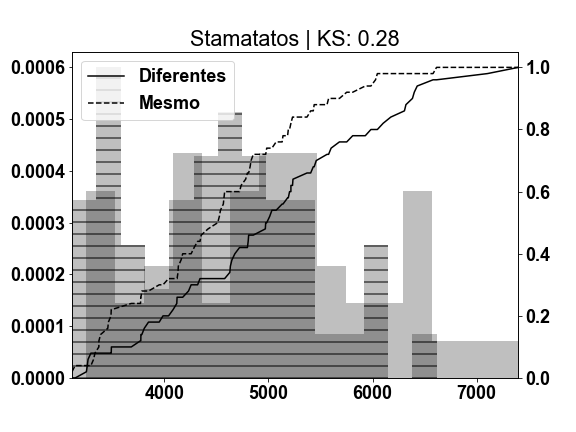
\includegraphics[width=.45\textwidth]{experimentoVerificacao/HDRIO_KS_spanish_Stamatatos.png} \vspace{0.3cm}
	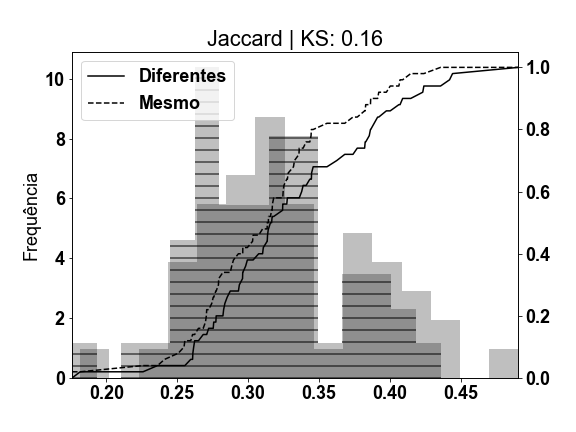
\includegraphics[width=.45\textwidth]{experimentoVerificacao/HDRIO_KS_spanish_Jaccard.png} \vspace{0.3cm}
	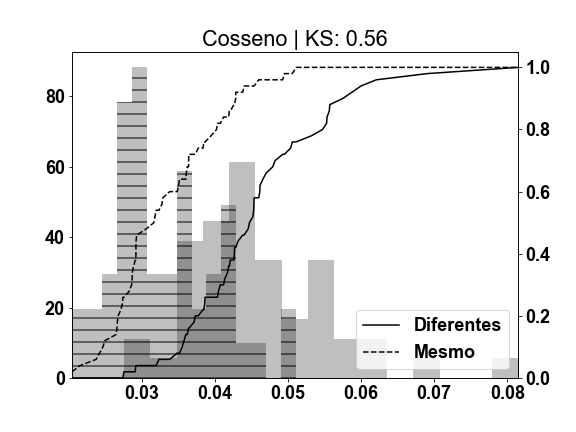
\includegraphics[width=.45\textwidth]{experimentoVerificacao/HDRIO_KS_spanish_Cosseno.png}
	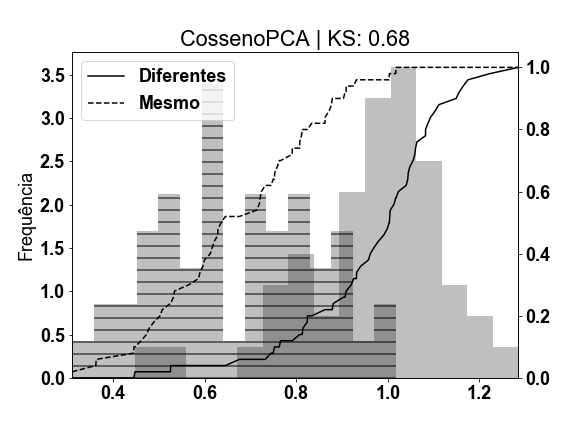
\includegraphics[width=.45\textwidth]{experimentoVerificacao/HDRIO_KS_spanish_CossenoPCA.png}
	\label{fig:exemplo}
\end{figure}
\end{column}
\begin{column}{0.37\textwidth}

\begin{itemize}
	\item Histograma para mesma autoria (tracejado).
	\item Histograma para autorias diferentes (liso).
	\item Distribuição acumuladas (linhas).
	\item Separação pela métrica Kolmogorov-Smirnov.
	\item Métricas AUC e acurácia.
\end{itemize}
\end{column}
\end{columns}


\end{frame}
\begin{frame}{Experimento 1: Verificação autoral}
\begin{block}{Modelo proposto 1 - MP1}
\begin{itemize}
\item As distâncias foram utilizadas como variáveis para o modelo.
\item Aplicado a normalização minmax.
\item Aplicado a regressão logística.
\end{itemize}
\end{block}
\begin{block}{Modelo proposto 2 - MP2}
\begin{itemize}
\item Os documentos conhecidos $C$ e de autoria desconhecidas $D$ foram unificados em um úncio BoW através da equação:
\begin{equation}
MP2\left ( C_{ij}, D_{ij} \right ) = \log\left ( 1 + \frac{\left ( C_{ij}-D_{ij} \right )^2}{C_{ij}+1} \right )
\label{eq:verificacao.mp2}
\end{equation}
\item Aplicado a normalização minmax.
\item Aplicado a regressão logística.
\end{itemize}		
\end{block}	
\end{frame}

\begin{frame}{Experimento 1: Verificação autoral}
\begin{table}[]
\caption{Verificação autoral - Resultados médios das métricas AUC e acurácia em 5-partições.}\selectFont
\begin{tabular}{l|cc|cc}
\toprule
\multirow{2}{*}{\bf Modelo} & \multicolumn{2}{c|}{\bf PAN2014 (EE e EM)} & \multicolumn{2}{c}  {\bf PAN2014{-}SP} \\ \cline{2-5}
& {\bf ROC}  &        {\bf Acurácia}         & {\bf ROC}  &      {\bf Acurácia}       \\ \hline
Jaccard                     &    0,60    &             0,56              &    0,57    &           0,52            \\
Cossenos                    &    0,63    &             0,50              &    0,88    &           0,77            \\
Cossenos\_PCA               &    0,63    &             0,55              & {\bf 0,92} &        {\bf 0,83}         \\
Keselj                      &    0,61    &             0,54              &    0,71    &           0,60            \\
Stamatatos                  &    0,60    &             0,55              &    0,59    &           0,54            \\ \hline
MP1 – Mix                   & {\bf 0,75} &          {\bf 0,67}           &    0,72    &           0,62            \\
MP2 – BOW                   &    0,62    &             0,53              & {\bf 0,93} &        {\bf 0,85}         \\ \bottomrule
\end{tabular} 
\label{tab.results.verificacao}
%\SourcePadrao
\end{table}

{\selectFont
PAN2014 (EE e EM) córpus com textos em língua inglesa, PAN2014{-}SP textos em língua espanhola.
}
\end{frame}


%*******************************************************************
\begin{frame}{Experimento 2: Atribuição Autoral}
\begin{block}{Publicação 2}
CUSTÓDIO, J. E.; PARABONI, I. EACH-USP Ensemble Cross-domain Authorship
Attribution: Notebook for PAN at CLEF 2018. In: CAPPELLATO, L. et al. (Ed.).
Working Notes Papers of the CLEF 2018 Evaluation Labs. [S.l.]: CLEF and CEUR-WS.org,
2018. (CEUR Workshop Proceedings). ISSN 1613-0073.
\end{block}

\begin{block}{Atribuição por aprendizado de máquina supervisionado}
\begin{itemize}
\item Tem-se um conjunto de documentos para os quais se sabe quem são os autores e um documento do qual deseja-se atribuir.
\item O classificador extrai a ``assinatura do estilo''.
\item Aspectos inconscientes, como a sintaxe, são mais importantes que a semântica.
\item O trabalho apresentado foi parte da participação da tarefa de AA da competição PAN-CLEF2018.
\end{itemize}
\end{block}
\end{frame}

\begin{frame}{Experimento 2: Atribuição Autoral}
\begin{block}{Baseline {\it Bas.PAN}}
Os organizadores forneceram um sistema {\it baseline} pelos com as seguintes características:
\begin{itemize}
\item N-gramas de caracteres de tamanho fixo.
\item Normalização no documento por TF.
\item Sem normalização no córpus.
\item Frequência mínima de 4 ocorrências.
\item Classificador SVM encapsulado nas estratégias um-contra-um e um-contra-todos.
\item Foi otimizado por {\it grid search} com validação cruzada com 5 partições, e os melhores parâmetros foram:
\begin{itemize}\selectFont
\item n-gramas de tamanho 4.
\item Frequência mínima de 5 documentos.
\item SVM com estratégia um-contra-todos.
\end{itemize}
\end{itemize}
\end{block}
\end{frame}

\begin{frame}{Experimento 2: Atribuição Autoral}
Dado nossas premissas, o sistema final PAN2018 para AA consistiu de um comitê que concatenou as fontes de informações em uma saída única.

\begin{figure}[]\selectFont
\caption{\selectFont Método proposto final}
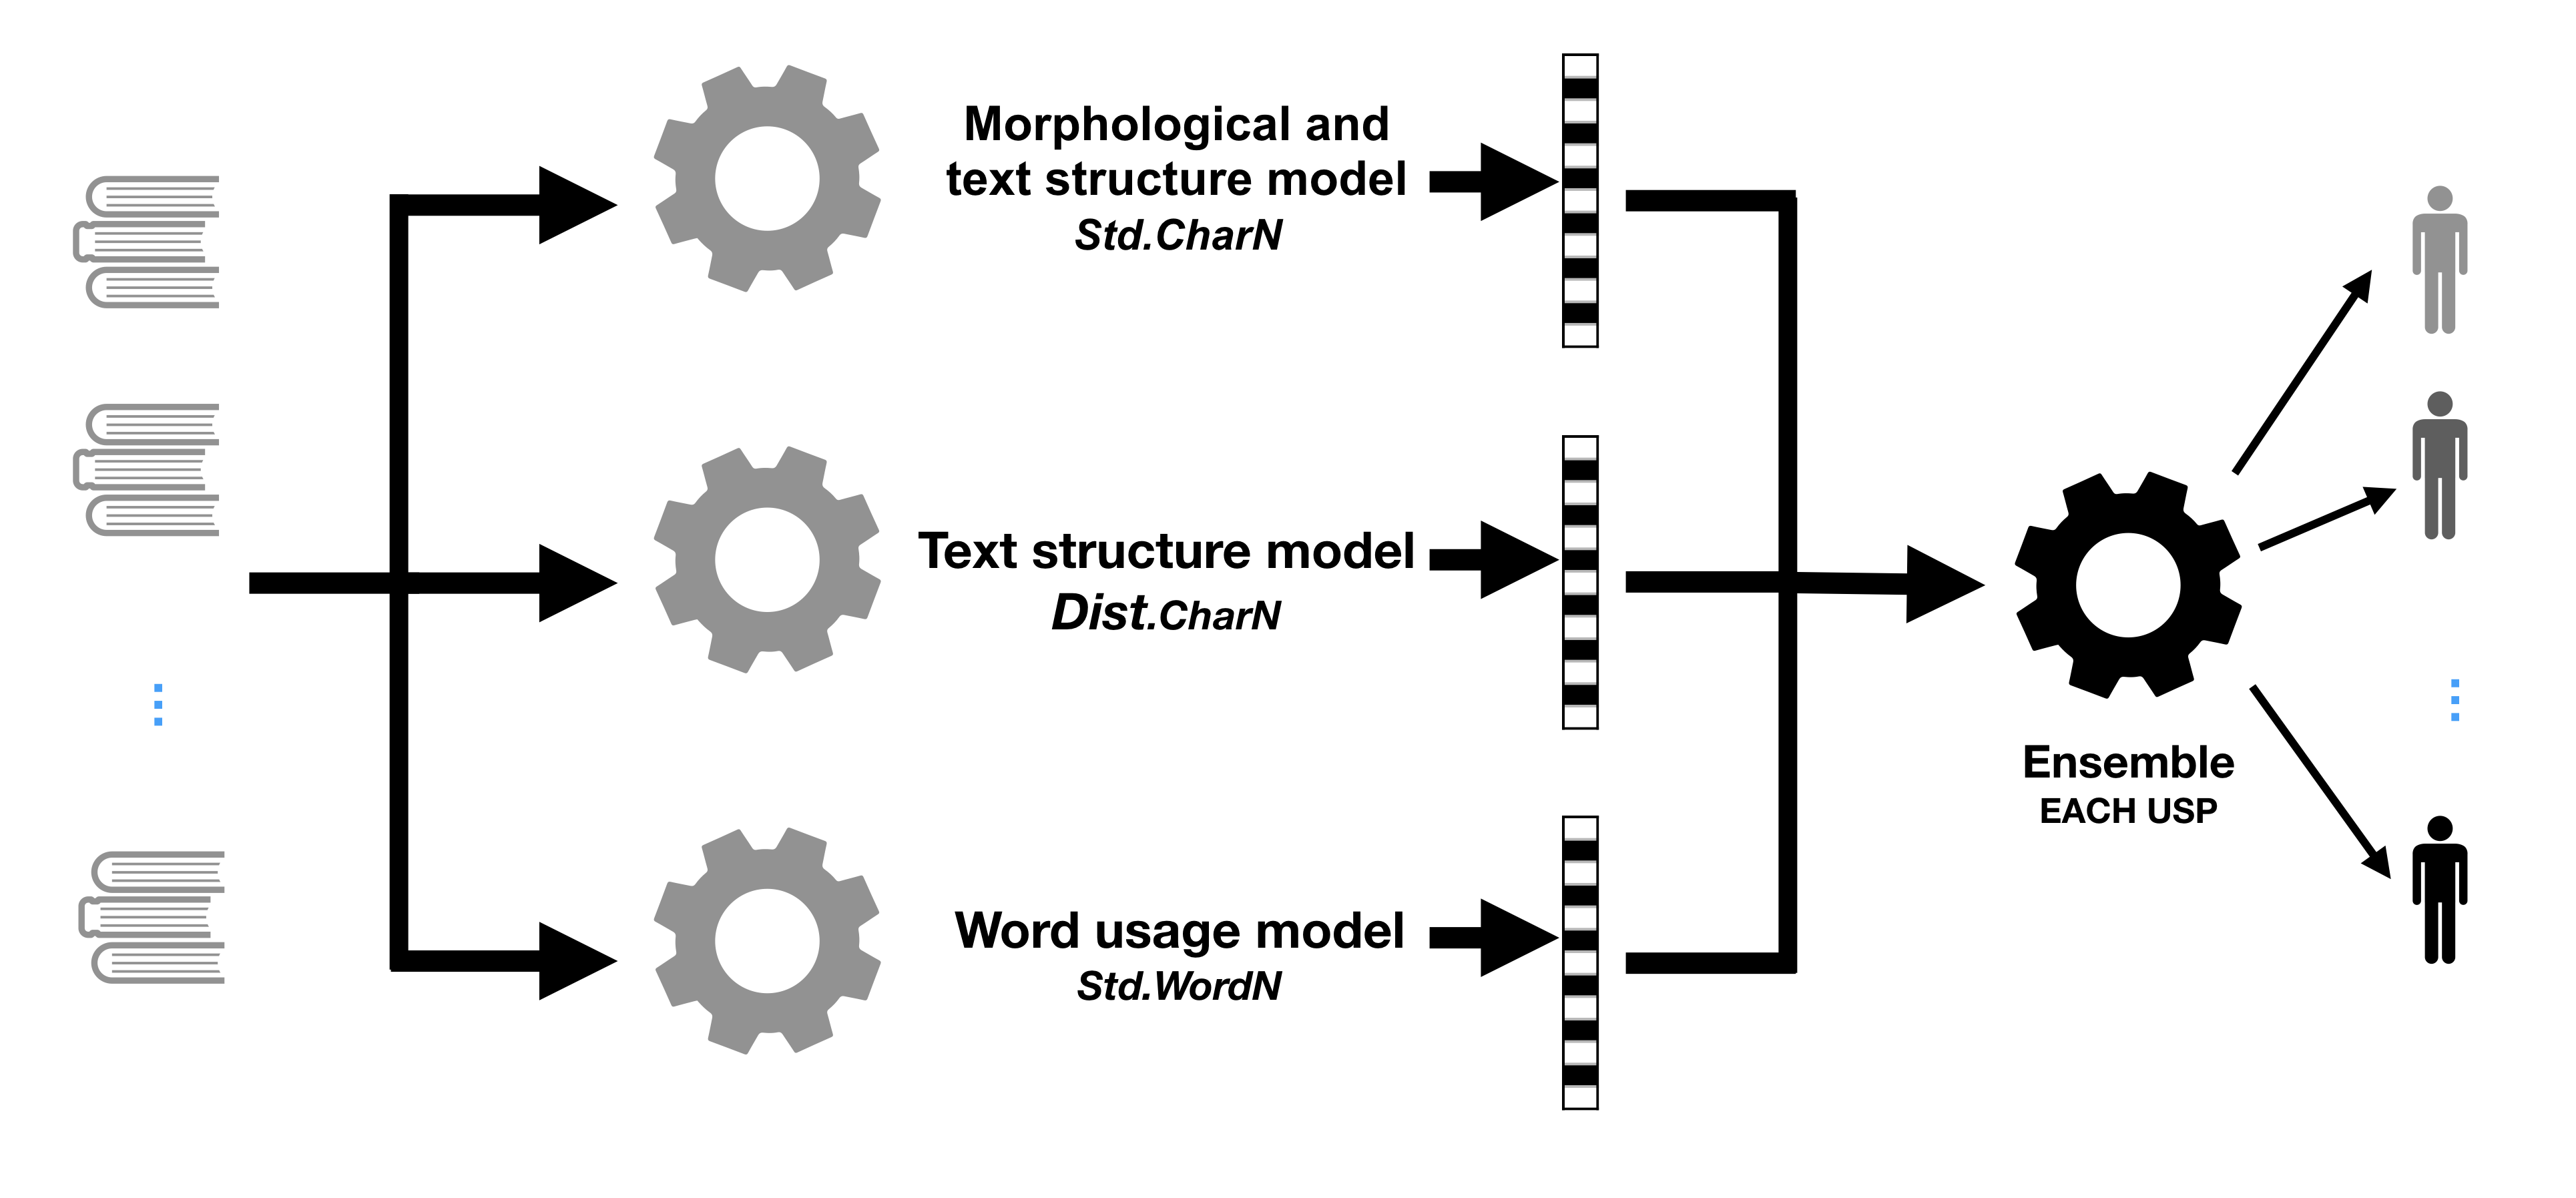
\includegraphics[width=.7\textwidth]{images/prop1_Diagramas.png}
\end{figure}

O sistema foi otimizado por {\it grid search} com validação cruzada de 5 partições.
\end{frame}

\begin{frame}{Experimento 2: Atribuição Autoral}
Premissa: O estilo de escrita de autor pode ser capturado através de diversas fontes de informação, como sintática, léxica e semântica.
\begin{block}{Método proposto {\it Std.word}}
Consistiu de um modelo BOW de n-gramas de palavras tradicional.
\end{block}
\begin{block}{Método proposto {\it Std.char}}
Consistiu de um modelo BOW de n-gramas de caracteres tradicional.
\end{block}
\begin{block}{Método proposto {\it Dist.char}}
Consistiu de um modelo BOW de n-gramas de caracteres onde são letras maiúscula e minúsculas sem acento são distorcidas, deixando a pontuação, espaços e letras com diacríticos.
\end{block}
\end{frame}

\begin{frame}{Experimento 2: Atribuição Autoral}
\selectFont
\setlength{\tabcolsep}{3pt}
\begin{table}[!htbp]
\centering
\caption{\selectFont Valores ótimos encontrados para PAN2018}
\begin{tabular}{m{2.2cm}m{4cm}m{4cm}}
\toprule
\textbf{Módulo} & \textbf{Parâmetros} & \textbf{Valores ótimos} \\ 
\midrule
\multirow{6}{2.2cm}{\bf Extração de características} & Faixa n-gram & 
\begin{tabular}[c]{@{}l@{ - }l@{}}
Std.charN &  Início=2 Fim=5\\
Dist.charN & Início=2 Fim=5\\
Std.WordN & Início=1 Fim=3\end{tabular}\\ 
& Freq. min. doc. & 0,05 \\ %\cline{2-3} 
& Freq. max. doc. & 1,0 \\ %\cline{2-3} 
& TF & Sublinear \\ %\cline{2-3} 
& IDF & Suavizado \\ %\cline{2-3} 
& Normalização no documento & L2 \\ 
\hline
{\bf Transformação} & PCA & 0,99 \\ 
\bottomrule
\end{tabular}
\label{tab.optimal}
\end{table}
\end{frame}

\begin{frame}{Experimento 2: Resultados obtidos em treinamento}

\setlength{\tabcolsep}{4pt}\selectFont
\begin{table}[!htbp]
\centering
\caption{\selectFont F1 para PAN-CLEF 2018 AA no córpus de desenvolvimento}
\begin{tabular}{ccc ccccc}
\bottomrule
{Problema} & {Língua} & {Autores} & {Bas.PAN} & {Std.charN} & {Dist.charN} & {Std.wordN} &   {Comitê}   \\ \midrule
01     &    EN    &    20     & 0,514     &    0,609    &    0,479     &    0,444    & {\bf 0,625}  \\
02     &    EN    &     5     & 0,626     &    0,535    &    0,333     &    0,577    & {\bf 0,673}  \\
03     &    FR    &    20     & 0,631     &    0,681    &    0,568     &    0,418    & {\bf 0,776}  \\
04     &    FR    &     5     & 0,747     &    0,719    &    0,586     &    0,572    & {\bf 0,820}  \\
05     &    IT    &    20     & 0,529     &    0,597    &    0,491     &    0,497    & {\bf 0,578}  \\
06     &    IT    &     5     & 0,614     &    0,623    &    0,595     &    0,520    & {\bf 0,663}  \\
07     &    PL    &    20     & 0,455     &    0,470    &    0,496     &    0,475    &   { 0,554}   \\
08     &    PL    &     5     & 0,703     & {\bf 0,948} &    0,570     &    {\bf 0,922}    &    0,922     \\
09     &    ES    &    20     & 0,709     & {\bf 0,774} &    0,589     &    0,616    &    0,701     \\
10     &    ES    &     5     & 0,593     &    0,778    &   {\bf 0,802} &    0,588    & {\bf 0,830}  \\ \bottomrule
Média    &          &           & 0,612     &    0,673    &    0,551     &    0,563    & {\bf 0,714 } \\ \bottomrule
\end{tabular}
\label{tab.results}
\end{table}
\end{frame}


\begin{frame}{Experimento 2: Resultados obtidos em produção}
\selectFont

Resultado geral apresentados pelos organizadores do PAN2018 \cite{aa-overview-2018}.

\setlength{\tabcolsep}{3pt}\selectFont
\begin{table}[]
\centering
\caption{\selectFont PAN-CLEF 2018 - 3 melhores equipes - por língua}
\begin{tabular}{m{5cm}cccccc}
	\toprule
	{\bf Equipe}                      & {\bf F1 Geral} &  {\bf EN}   &  {\bf FR}   &  {\bf IT}   & {\bf PL} &  {\bf ES}   \\ \midrule
	\citeonline{custodioParaboni2018} &  {\bf 0,685}   &    0,744    & {\bf 0,668} &    0,676    &  0,482   & {\bf 0,856} \\
	\citeonline{Murauer2018}          &     0,643      & {\bf 0,762} &    0,607    &    0,663    &  0,450   &    0,734    \\
	\citeonline{Halvani2018}          &     0,629      &    0,679    &    0,536    & {\bf 0,752} &  0,426   &    0,751    \\
	PAN18-BASELINE                    &     0,584      &    0,697    &    0,585    &    0,605    &  0,419   &    0,615    \\ \bottomrule
\end{tabular}

\caption{\selectFont PAN-CLEF 2018 - 3 melhores equipes - por língua}
\begin{tabular}{m{5cm}cccc}
	\toprule
	{}                                &     \multicolumn{4}{c}{\bf Quantidade de autores}     \\ \cline{2-5}
	{\bf Equipe}                      &  {\bf 20 }  &  {\bf 15 }  &  {\bf 10 }  &  {\bf 5 }   \\ \midrule
	\citeonline{custodioParaboni2018} & {\bf 0,648} & {\bf 0,676} & {\bf 0,739} & {\bf 0,677} \\
	\citeonline{Murauer2018}          &    0,609    &    0,642    &    0,680    &    0,642    \\
	\citeonline{Halvani2018}          &    0,609    &    0,605    &    0,665    &    0,636    \\
	PAN18-BASELINE                    &    0,546    &    0,532    &    0,595    &    0,663    \\ \bottomrule
\end{tabular}
\label{tab.experimento1.resultados.por.autores}
\end{table}
\end{frame}

\section{Projeto de pesquisa}

\begin{frame}{Projeto de pesquisa}
	\begin{alertblock}{Projeto de pesquisa }
	\end{alertblock}
\end{frame}



\begin{frame} {Projeto - Hipóteses}

Este trabalho considera as seguintes hipóteses:

\begin{block}{H1:} O uso de modelos independentes de idioma do tipo de distorção textual permite filtrar aspectos específicos do texto, e a combinação de diversos tipos de distorção pode aumentar o desempenho de sistemas de AA.
\end{block}

\begin{block}{H2:} O uso de modelos dependentes de idioma do tipo {\it part-of-speech} extraídos por anotadores baseados em aprendizado profundo pode aumentar o desempenho de sistemas de AA.
\end{block}


\begin{block}{H3:} O uso de modelos dependentes de idioma do tipo representação distribuída ({\it embeddings}) pode aumentar o desempenho de sistemas de AA.
\end{block}

\end{frame}

\begin{frame}{Projeto - Objetivo}
\begin{block}{Objetivo Geral}
O objetivo geral deste trabalho é enriquecer modelos de atribuição autoral de texto digitais com conjunto fechado de autores utilizando conhecimentos dependentes e independentes de idioma combinados com técnicas de aprendizados de máquina, de modo a obter resultados superiores ao estabelecido em trabalhos anteriores.
\end{block}
\end{frame}


\begin{frame}{Projeto - Conjunto de dados e Avaliação}

\begin{block}{Avaliação das hipóteses}
	\begin{itemize}
		\item Comparação com {\it baselines} pertinentes, como o modelo apresentado em \citeonline{custodioParaboni2018}.
		\item Serão utilizadas as medidas tradicionais de AM, como {\it medida F}, acurácia, auroc e outros.
		\item Espera-se que o resultado médio seja superior ao dos modelos de {\it baseline}.
	\end{itemize}
\end{block}

\setlength{\tabcolsep}{4pt}\selectFont
\begin{table}[!htbp]
	\centering
	\caption{Córpus para avaliação dos métodos de AA}
	\begin{tabular}{l|rll}
		\toprule
		Córpus       & No. Autores & Idioma             & Domínio/Gênero \\ \midrule
		PAN-CLEF2014 &           - & EN, ES, DU, GR     & NV, AR, RV, ES \\ \hline
		PAN-CLEF2018 &          20 & EN, ES, FR, IT, PL & NV             \\ \hline
		RCV1         &          50 & EN                 & AR             \\ \hline
		Nus-SMS      &         116 & EN                 & SMS            \\ \hline
		b5-post      &       1.019 & PT-Br              & Facebook       \\ \hline
		BlogSet-BR   &       4.331 & PT-Br              & AR             \\ \bottomrule
	\end{tabular}
	\label{tab.results}
\end{table}

\end{frame}

\begin{frame}{Projeto - Escopo e limitações}
	Este projeto de pesquisa se limita
	\begin{itemize}
		\item ao estudo das técnicas de distorção textual
		\item ao estudo das técnicas de anotações linguísticas
		\item ao estudo das técnicas de representação distribuída
		\item e utilizará métodos de aprendizado de máquina.
		\item aos idiomas considerados primordialmente são inglês e português brasileiro.
	\end{itemize}

	Não serão considerados
	\begin{itemize}
		\item  modelos computacionais baseados em grafos, redes complexas e modelos de compressão.
	\end{itemize}
\end{frame}


\begin{frame}{Projeto - Atividades}

\begin{enumerate}
	\item {\bf Revisão bibliográfica} Concluído.
	
	\item {\bf Participação na PAN-CLEF 2018} Concluído.
	
	\item {\bf Preparação dos dados} Concluído.
	
	\item {\bf Modelos independentes de idioma} Estudo dos tipo de distorção textual, construção dos modelos computacionais e refinamentos específicos.
	
	\item {\bf Modelos baseados em anotações} Estudo dos pacotes para anotações POS, como NLTK\footnote{Disponível em  \url{https://www.nltk.org/}} e Spacy, construção dos modelos computacionais e refinamentos específicos.
	
	\item {\bf Modelos baseados em {\it embeddings}} Preparação de bases de dados de {\it embeddings}, estudo de {\it embeddings} específicos para AA, construção de modelos computacionais e refinamentos.
	
	\item {\bf Refinamentos} 
	
	\item {\bf Avaliação}
	
	\item {\bf Redação da dissertação} 
	
	\item {\bf Divulgação} 
\end{enumerate}
\end{frame}

\begin{frame}{Projeto - Cronograma}


\setlength{\tabcolsep}{4pt}\selectFont
\begin{table}[]
	\centering
	\caption{Cronograma}
		\begin{tabular}{|l|l|l|l|l|l|l|l|l|l|l|l|l|l|}
			\toprule
			                                         & \multicolumn{7}{c|}{2018}      & \multicolumn{6}{c|}{2019} \\ \midrule
			Atividades                               & 1-6 & 7 & 8 & 9 & 10 & 11 & 12 & 1 & 2 & 3 & 4 & 5 & 6     \\ \hline
			01. Revisão bibliográfica                & x   & x & x & x & x  &    &    &   &   &   &   &   &       \\ \hline
			02. Participação PAN-CLEF2018            & x   &   &   &   &    &    &    &   &   &   &   &   &       \\ \hline
			03. Preparação dos dados                 & x   & x &   &   &    & x  &    &   &   &   &   &   &       \\ \hline
			04. Modelos independentes de idioma      &     &   &   &   &    & x  & x  & x &   &   &   &   &       \\ \hline
			05. Modelos baseados em anotações        &     & x &   &   &    & x  & x  & x &   &   &   &   &       \\ \hline
			06. Modelos baseados em {\it embeddings} &     & x &   &   &    &    &    & x & x &   &   &   &       \\ \hline
			07. Refinamentos                         &     &   &   &   &    &    &    & x & x & x &   &   &       \\ \hline
			08. Avaliação final                      &     &   &   &   &    &    &    &   &   & x &   &   &       \\ \hline
			09. Redação da dissertação               &     &   &   &   &    &    &    &   &   & x & x & x &       \\ \hline
			10. Divulgação                           &     &   &   &   &    &    &    &   &   &   &   & x & x     \\ \bottomrule
		\end{tabular}
	\end{table}
\end{frame}




%=======================================
\section{Referências}
\begin{frame}[allowframebreaks]{Referências}

%\bibliographystyle{abbrv}
\bibliography{bibliografia}

\end{frame}



\end{document}
